\documentclass[11pt,letterpaper]{article}

% Compilar con lualatex
\usepackage{fontspec}
\usepackage[spanish,es-noquoting,es-nodecimaldot]{babel}
\setmainfont{Times New Roman}
\setmonofont{lmmono10-regular.otf}[BoldFont=lmmonolt10-bold.otf, ItalicFont=lmmono10-italic.otf]  % código
\usepackage[margin=2.5cm]{geometry}
\usepackage{setspace}
\usepackage{graphicx}
\usepackage{float}
\usepackage{booktabs}
\usepackage{array}
\usepackage{xcolor}
\usepackage{listings}
\usepackage{caption}
\usepackage{xurl}
\usepackage[hidelinks]{hyperref}

\onehalfspacing
\setlength{\parindent}{0pt}
\setlength{\parskip}{2pt}

\captionsetup{font=small, labelfont=bf, skip=3pt}
\setlength{\intextsep}{5pt}   % espacio alrededor de tablas y figuras
\usepackage{titlesec}
\usepackage{needspace}
\titlespacing*{\section}{0pt}{5pt}{1pt}
\titlespacing*{\subsection}{0pt}{6pt}{1pt}

\definecolor{fondocodigo}{RGB}{246,247,249}
\definecolor{bordecodigo}{RGB}{200,205,212}

\lstset{
  basicstyle=\ttfamily\footnotesize\setstretch{1},
  backgroundcolor=\color{fondocodigo},
  frame=single,
  rulecolor=\color{bordecodigo},
  framesep=4pt,
  breaklines=true,
  columns=fullflexible,
  keepspaces=true,
  showstringspaces=false,
  aboveskip=4pt,
  belowskip=4pt,
  inputencoding=utf8,
  extendedchars=true,
  literate={á}{{\'a}}1 {é}{{\'e}}1 {í}{{\'i}}1 {ó}{{\'o}}1 {ú}{{\'u}}1 {ñ}{{\~n}}1,
}
\renewcommand{\lstlistingname}{Código}

\newcommand{\shell}[1]{\texttt{\small #1}}
\newcommand{\referencia}[1]{\noindent\hangindent=1.27cm\hangafter=1 #1\par\vspace{4pt}}

\begin{document}

\begin{center}
  {\Large\bfseries Actividad Individual\\
  Código de experimentación base con MLflow}

  \vspace{2pt}
  {\small Gerardo González Martínez, A01840096, 11 de octubre de 2026}

  \vspace{2pt}
  {\small \url{https://github.com/gerardoglezmart/mna-tc5061-actividad3-experimentacion-mlflow}}
\end{center}

\vspace{-6pt}
\hrule
\vspace{4pt}

\section*{1. Migración del notebook a un script}

Carga, preprocesamiento, entrenamiento y evaluación pasaron del notebook de la semana 3 a
funciones con una sola responsabilidad, en un proyecto generado con Cookiecutter Data Science
(\shell{ccds}). \shell{main.py} las ejecuta en orden (Código 1) y el notebook queda solo para
la exploración de datos.

\begin{table}[H]
\centering\small
\begin{tabular}{@{}lll@{}}
\toprule
\textbf{Etapa} & \textbf{Archivo} & \textbf{Funciones} \\
\midrule
Carga de datos & \shell{wine\_quality/dataset.py} & \shell{cargar\_datos} \\
Preprocesamiento & \shell{wine\_quality/dataset.py} & \shell{limpiar\_datos}, \shell{dividir\_datos} \\
Entrenamiento & \shell{wine\_quality/modeling/train.py} & \shell{construir\_modelo} \\
Evaluación & \shell{wine\_quality/modeling/evaluate.py} & \shell{evaluar}, \shell{guardar\_artefactos} \\
Ejecución y registro & \shell{main.py} & \shell{leer\_argumentos}, \shell{main} \\
\bottomrule
\end{tabular}
\end{table}

\par\noindent\begin{minipage}{\linewidth}
\lstinputlisting[language=Python, firstline=42, lastline=50, firstnumber=42, numbers=left,
  numberstyle=\tiny\color{gray}, caption={\shell{main.py}: orden de ejecución con las
  funciones de cada etapa.}]{../main.py}
\end{minipage}\par\vspace{6pt}

\Needspace{10\baselineskip}
\section*{2. Parametrización de la ejecución}

Tres hiperparámetros y la semilla se exponen con \shell{argparse}, con valor por defecto y
ayuda descriptiva. Sin argumentos se reproduce el baseline de la semana 3 (Figura 1).

\begin{table}[H]
\centering\small
\begin{tabular}{@{}lll@{}}
\toprule
\textbf{Argumento} & \textbf{Default} & \textbf{Descripción} \\
\midrule
\shell{-{}-C} & 1.0 & Inverso de la fuerza de regularización \\
\shell{-{}-class-weight} & none & \shell{balanced} da más peso a la clase minoritaria \\
\shell{-{}-max-iter} & 1000 & Máximo de iteraciones del optimizador lbfgs \\
\shell{-{}-seed} & 42 & Semilla de la partición train/test \\
\bottomrule
\end{tabular}
\end{table}

\par\noindent\begin{minipage}{\linewidth}
Comando exacto, desde la raíz del repositorio y con el ambiente activado:
\begin{lstlisting}
python main.py --class-weight balanced --C 1.0
\end{lstlisting}
\end{minipage}\par

\begin{figure}[H]
\centering
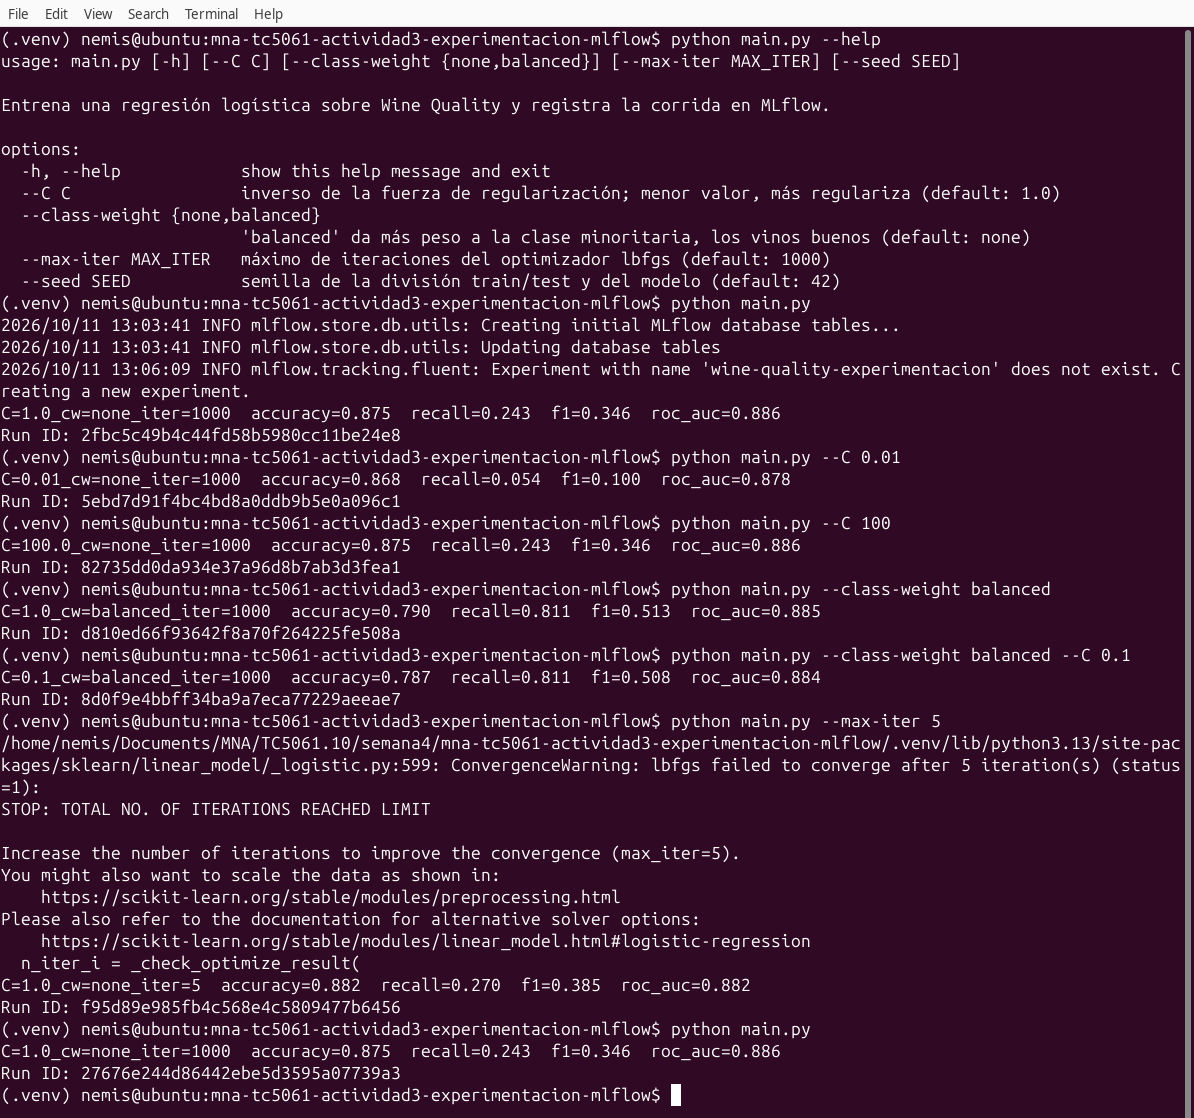
\includegraphics[width=0.92\linewidth]{figures/01_terminal_corridas.png}
\caption{\shell{python main.py -{}-help} con la ayuda de cada argumento, la corrida
sin argumentos y las siete corridas. La primera y la última imprimen las mismas métricas.}
\end{figure}

\Needspace{10\baselineskip}
\section*{3. Instrumentación con MLflow Tracking}

Todo el registro ocurre dentro de un \shell{mlflow.start\_run()} (Código 2, Figuras 2 y 3).

\begin{table}[H]
\centering\small
\begin{tabular}{@{}ll@{}}
\toprule
\textbf{Requisito} & \textbf{Implementación} \\
\midrule
Hiperparámetros con \shell{log\_param} & \shell{C}, \shell{class\_weight}, \shell{max\_iter} y \shell{seed} \\
Métricas con \shell{log\_metric} & accuracy, recall, F1 y ROC-AUC \\
Artefactos con \shell{log\_artifact} & \shell{matriz\_confusion.png} y \shell{classification\_report.txt} \\
Modelo con \shell{mlflow.sklearn.log\_model} & \shell{Pipeline} de \shell{StandardScaler} y \shell{LogisticRegression} \\
\bottomrule
\end{tabular}
\end{table}

\par\noindent\begin{minipage}{\linewidth}
\lstinputlisting[language=Python, linerange={53-53,56-64}, consecutivenumbers=false,
  numbers=left, numberstyle=\tiny\color{gray}, caption={\shell{main.py}: registro de la
  corrida dentro de \shell{mlflow.start\_run()}.}]{../main.py}
\end{minipage}\par\vspace{6pt}

\begin{figure}[H]
\centering
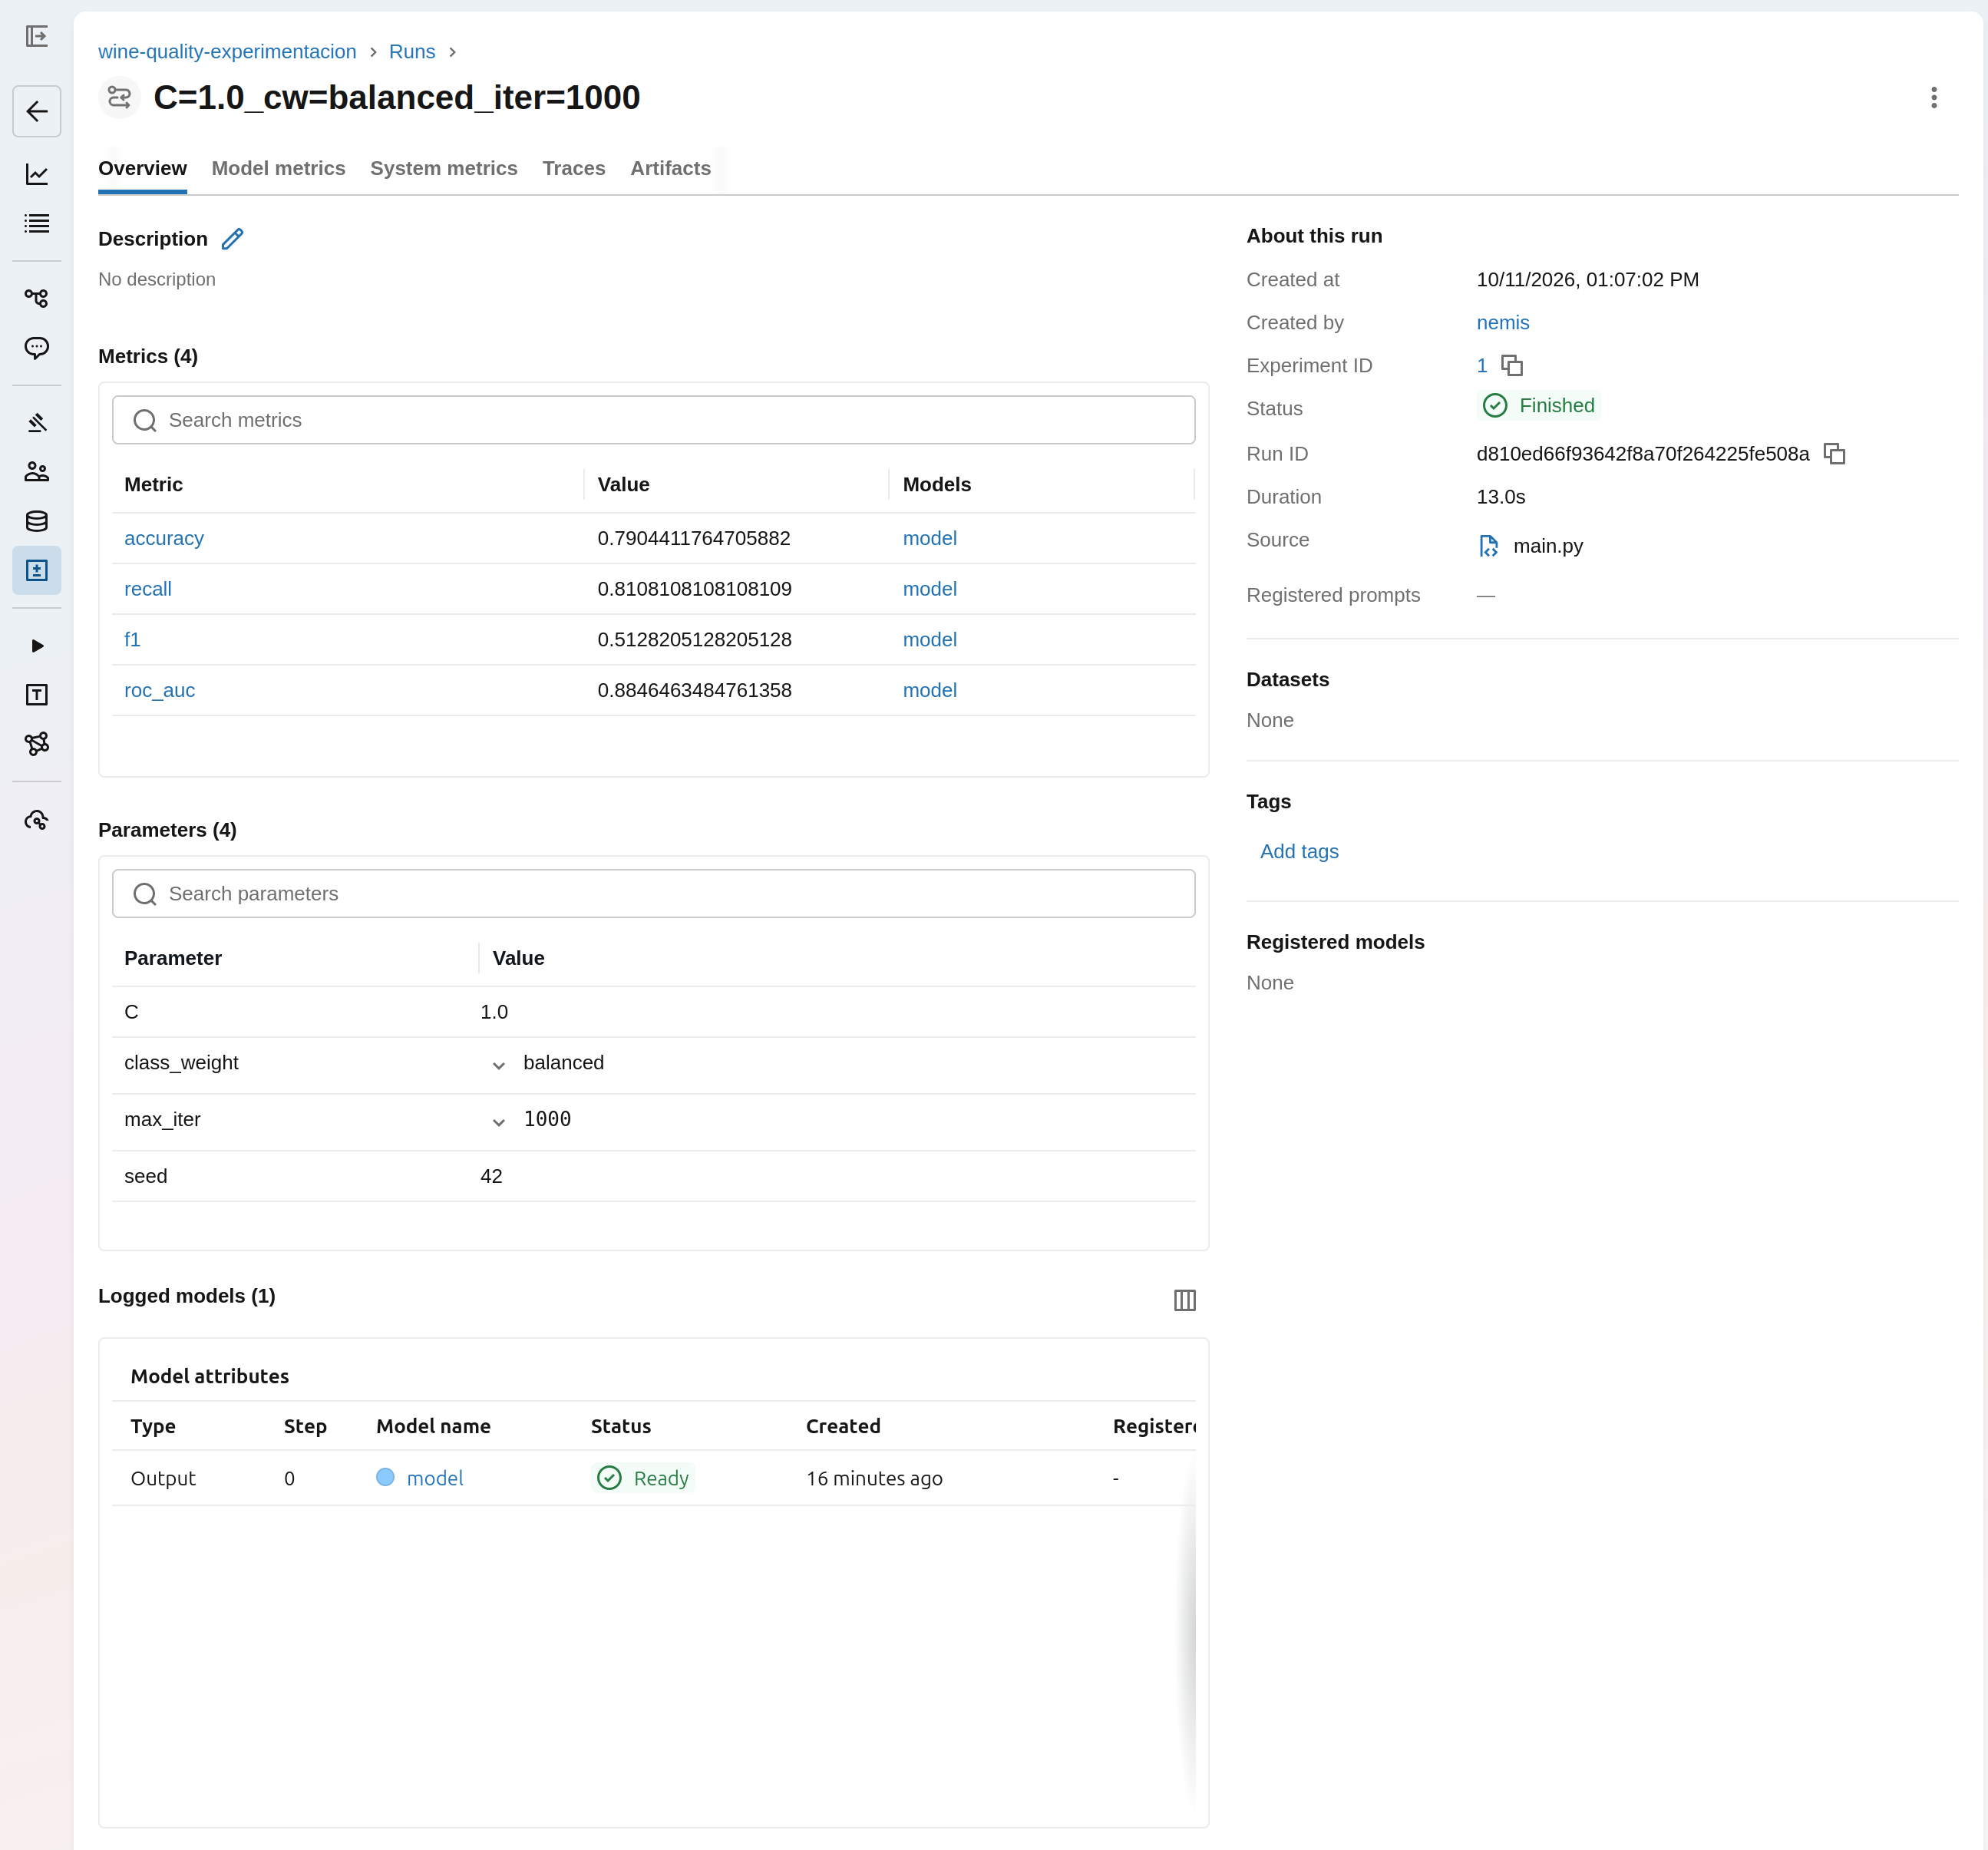
\includegraphics[width=0.80\linewidth]{figures/02_mlflow_detalle_corrida.png}
\caption{Detalle de la corrida 4 en MLflow: métricas (\shell{log\_metric}), parámetros
(\shell{log\_param}) y el modelo registrado (\shell{log\_model}).}
\end{figure}

\begin{figure}[H]
\centering
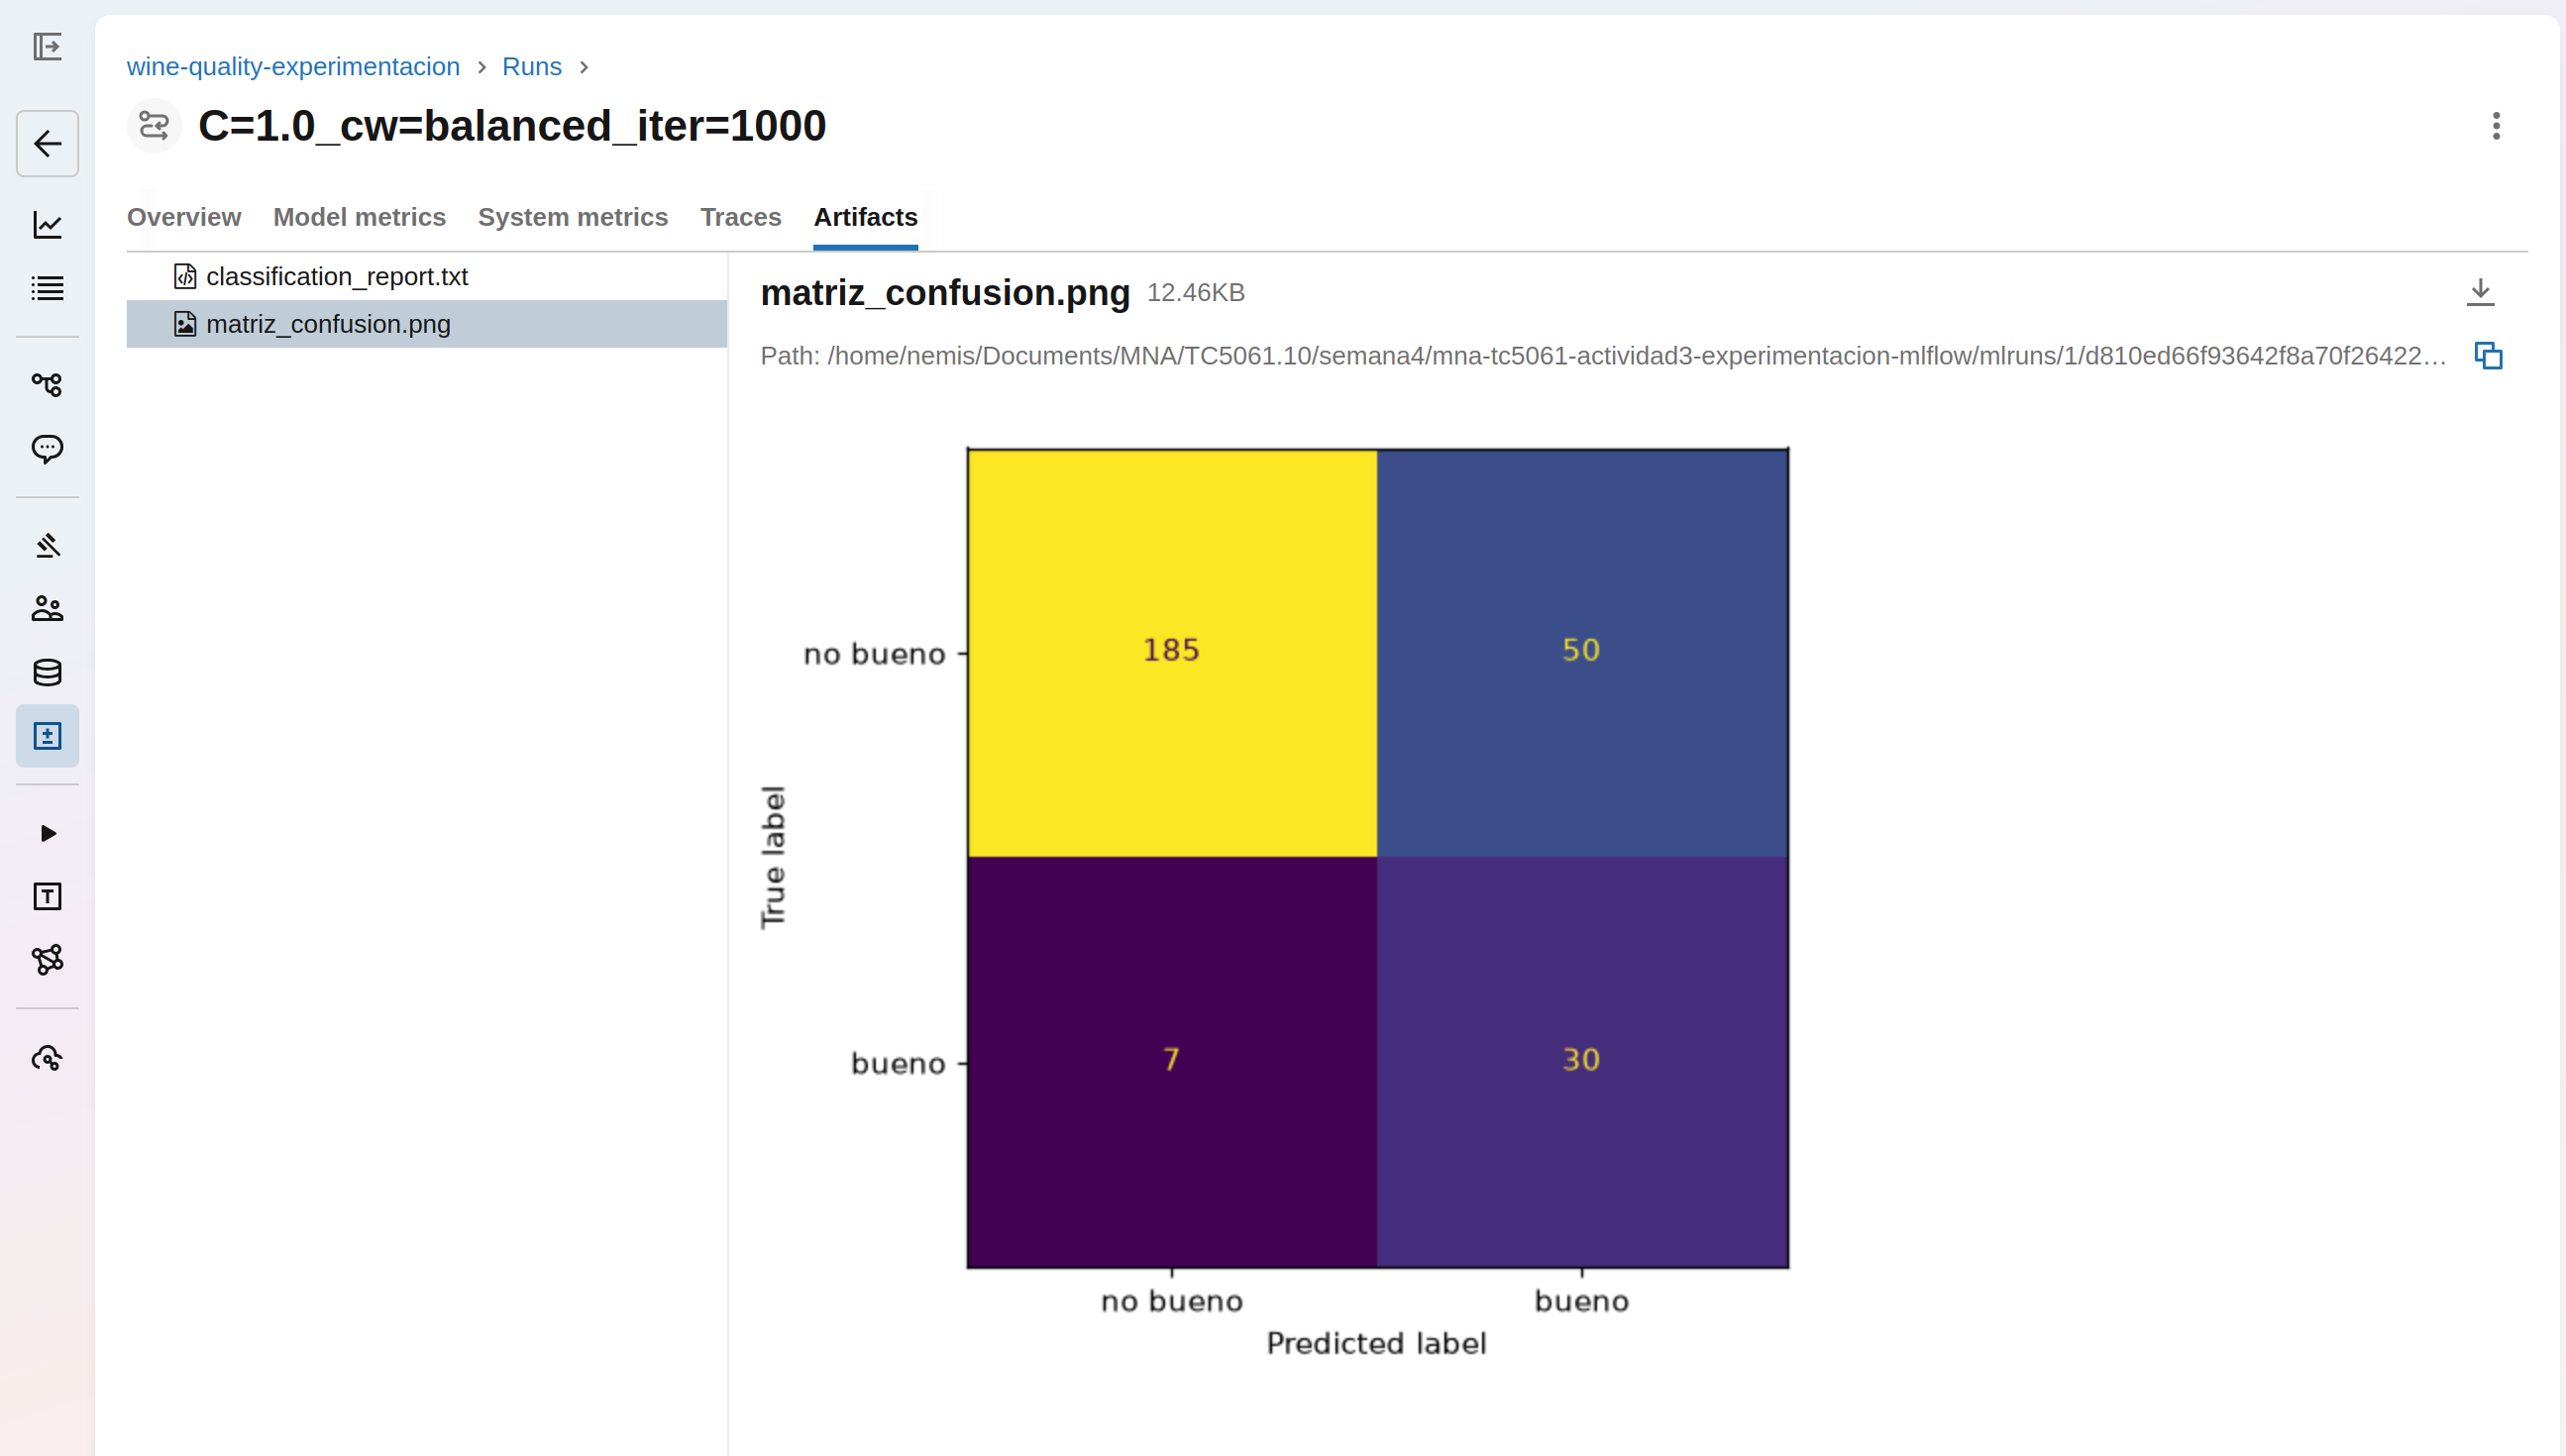
\includegraphics[width=0.80\linewidth]{figures/03_mlflow_artefactos.png}
\caption{Pestaña \textit{Artifacts} de la misma corrida: la matriz de confusión y el
classification report (\shell{log\_artifact}).}
\end{figure}

\Needspace{10\baselineskip}
\section*{4. Ejecución y comparación de corridas}

Siete corridas en el experimento \shell{wine-quality-experimentacion}, contrastadas en MLflow
(Figura 4).

\begin{table}[H]
\centering\small
\begin{tabular}{@{}clcccc@{}}
\toprule
\textbf{\#} & \textbf{Argumentos} & \textbf{accuracy} & \textbf{recall} & \textbf{F1} & \textbf{ROC-AUC} \\
\midrule
1 & por defecto (C=1, sin pesos, 1000 iteraciones) & 0.875 & 0.243 & 0.346 & 0.886 \\
2 & \shell{-{}-C 0.01} & 0.868 & 0.054 & 0.100 & 0.878 \\
3 & \shell{-{}-C 100} & 0.875 & 0.243 & 0.346 & 0.886 \\
4 & \shell{-{}-class-weight balanced} & 0.790 & \textbf{0.811} & \textbf{0.513} & 0.885 \\
5 & \shell{-{}-class-weight balanced -{}-C 0.1} & 0.787 & 0.811 & 0.508 & 0.884 \\
6 & \shell{-{}-max-iter 5} & 0.882 & 0.270 & 0.385 & 0.882 \\
7 & por defecto, repetida & 0.875 & 0.243 & 0.346 & 0.886 \\
\bottomrule
\end{tabular}
\end{table}

\begin{figure}[H]
\centering
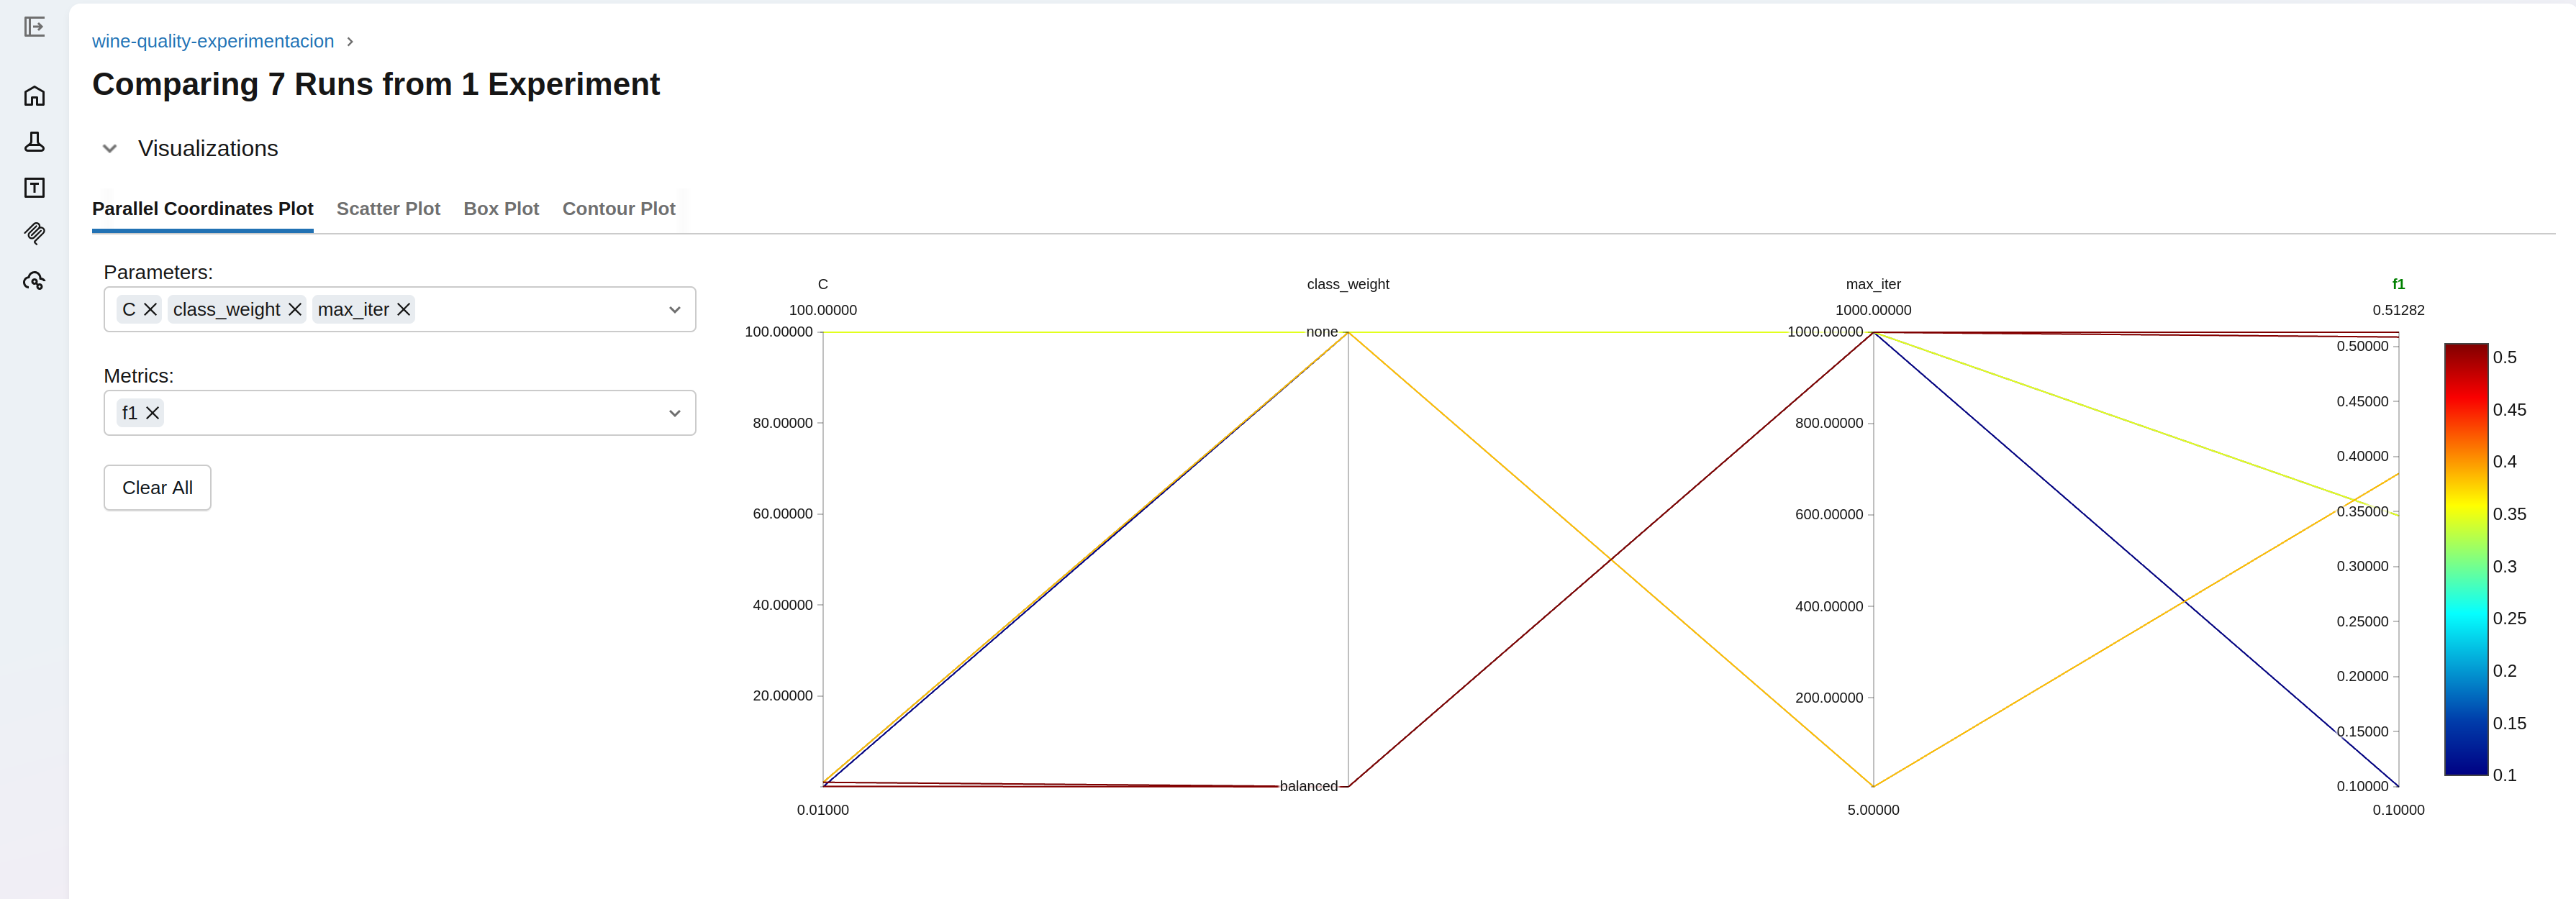
\includegraphics[width=\linewidth]{figures/04_mlflow_comparacion.png}
\caption{Vista de comparación de MLflow con las siete corridas del experimento
\shell{wine-quality-experimentacion}, en coordenadas paralelas coloreadas por F1.}
\end{figure}

\Needspace{10\baselineskip}
\section*{5. Fijación de la semilla y dependencias}

La semilla controla la partición estratificada de \shell{train\_test\_split}. También se pasa
a \shell{LogisticRegression}, pero con el solver lbfgs ese parámetro no interviene. La corrida 7
repite la 1 y sus métricas coinciden sin redondear (Tabla 1, exportada de MLflow con sus IDs).
Entorno: Ubuntu 24.04, Python 3.13.15 y las versiones fijadas en \shell{requirements.txt}
(Código 3), entre ellas mlflow 3.16.1 y scikit-learn 1.9.1.

\par\noindent\begin{minipage}{\linewidth}
\lstinputlisting[firstline=1, lastline=9, caption={\shell{requirements.txt} con las
versiones utilizadas.}]{../requirements.txt}
\end{minipage}\par\vspace{6pt}

\begin{table}[H]
\centering\small
\caption*{\textbf{Tabla 1:} Métricas sin redondear de las corridas 1 y 7, exportadas
de MLflow con \shell{mlflow.search\_runs} (las siete corridas están en
\shell{reports/corridas\_mlflow.csv}).}
\begin{tabular}{@{}lll@{}}
\toprule
 & \textbf{Corrida 1} & \textbf{Corrida 7} \\
\midrule
Run ID & \shell{2fbc5c49b4c44fd58b5980cc11be24e8} & \shell{27676e244d86442ebe5d3595a07739a3} \\
Argumentos & por defecto & por defecto \\
accuracy & 0.875 & 0.875 \\
recall & 0.24324324324324326 & 0.24324324324324326 \\
F1 & 0.34615384615384615 & 0.34615384615384615 \\
ROC-AUC & 0.88602645198389884 & 0.88602645198389884 \\
\bottomrule
\end{tabular}
\end{table}

\Needspace{10\baselineskip}
\section*{6. Análisis de resultados}

\textbf{Mejor configuración.} Entre las configuraciones probadas y en esta partición, la mejor
por F1 es la corrida 4, \shell{-{}-class-weight balanced} con C=1 (Figura 5): el F1 sube de 0.346
a 0.513.
El recall pasa de 0.243 a 0.811 (30 de 37 vinos buenos), pero la precisión positiva es de
37.5\,\%: de los 80 vinos que marca como buenos, 50 no lo son. Ese es el costo del recall y
la razón de que el accuracy baje a 0.790. El ROC-AUC parecido (0.886 contra 0.885) indica una
capacidad de discriminación similar. \shell{class\_weight} cambia el ajuste del modelo al dar
más peso a los vinos buenos, y el umbral de decisión sigue en 0.5.

\textbf{Hiperparámetro más influyente.} Depende de cómo se mida. \shell{class\_weight=balanced}
produjo la mayor mejora de F1 (+0.167). El mayor cambio absoluto lo produjo
\shell{C=0.01} (−0.246, F1 de 0.100), porque la regularización fuerte casi elimina las
predicciones positivas. Entre C=1 y C=100 se mantuvieron las métricas y las clases predichas,
aunque cambiaron las probabilidades. lbfgs convergió en 12 iteraciones (baseline), 7 (C=0.01)
y 13 (C=100 y balanceadas), así que \shell{max\_iter=1000} no limitó el ajuste. Con \shell{max\_iter=5} no hubo convergencia y su F1 de 0.385 corresponde a un modelo
incompleto, no a una configuración recomendable. Estas conclusiones valen solo para las siete
configuraciones probadas.

\textbf{Limitaciones.} El conjunto de prueba tiene 37 vinos buenos, así que esta evaluación no
permite establecer una superioridad estable entre configuraciones cercanas: entre las dos
balanceadas solo cambia un falso positivo (50 frente a 51). Además, la configuración se eligió
con el mismo conjunto de prueba, lo que hace optimista la estimación. Validación cruzada, otros
umbrales y otros modelos quedan como mejoras.

Más allá de qué configuración ganó, lo que me deja esta actividad es otra forma de trabajar.
En la semana 3 los resultados dependían de correr las celdas en el orden correcto y de
acordarme de qué había cambiado. Ahora cada corrida queda guardada con sus parámetros, sus
métricas y su modelo, y cualquiera puede repetirla con un solo comando. Eso es lo que permite
comparar con confianza y no solo con intuición.

\begin{figure}[H]
\centering
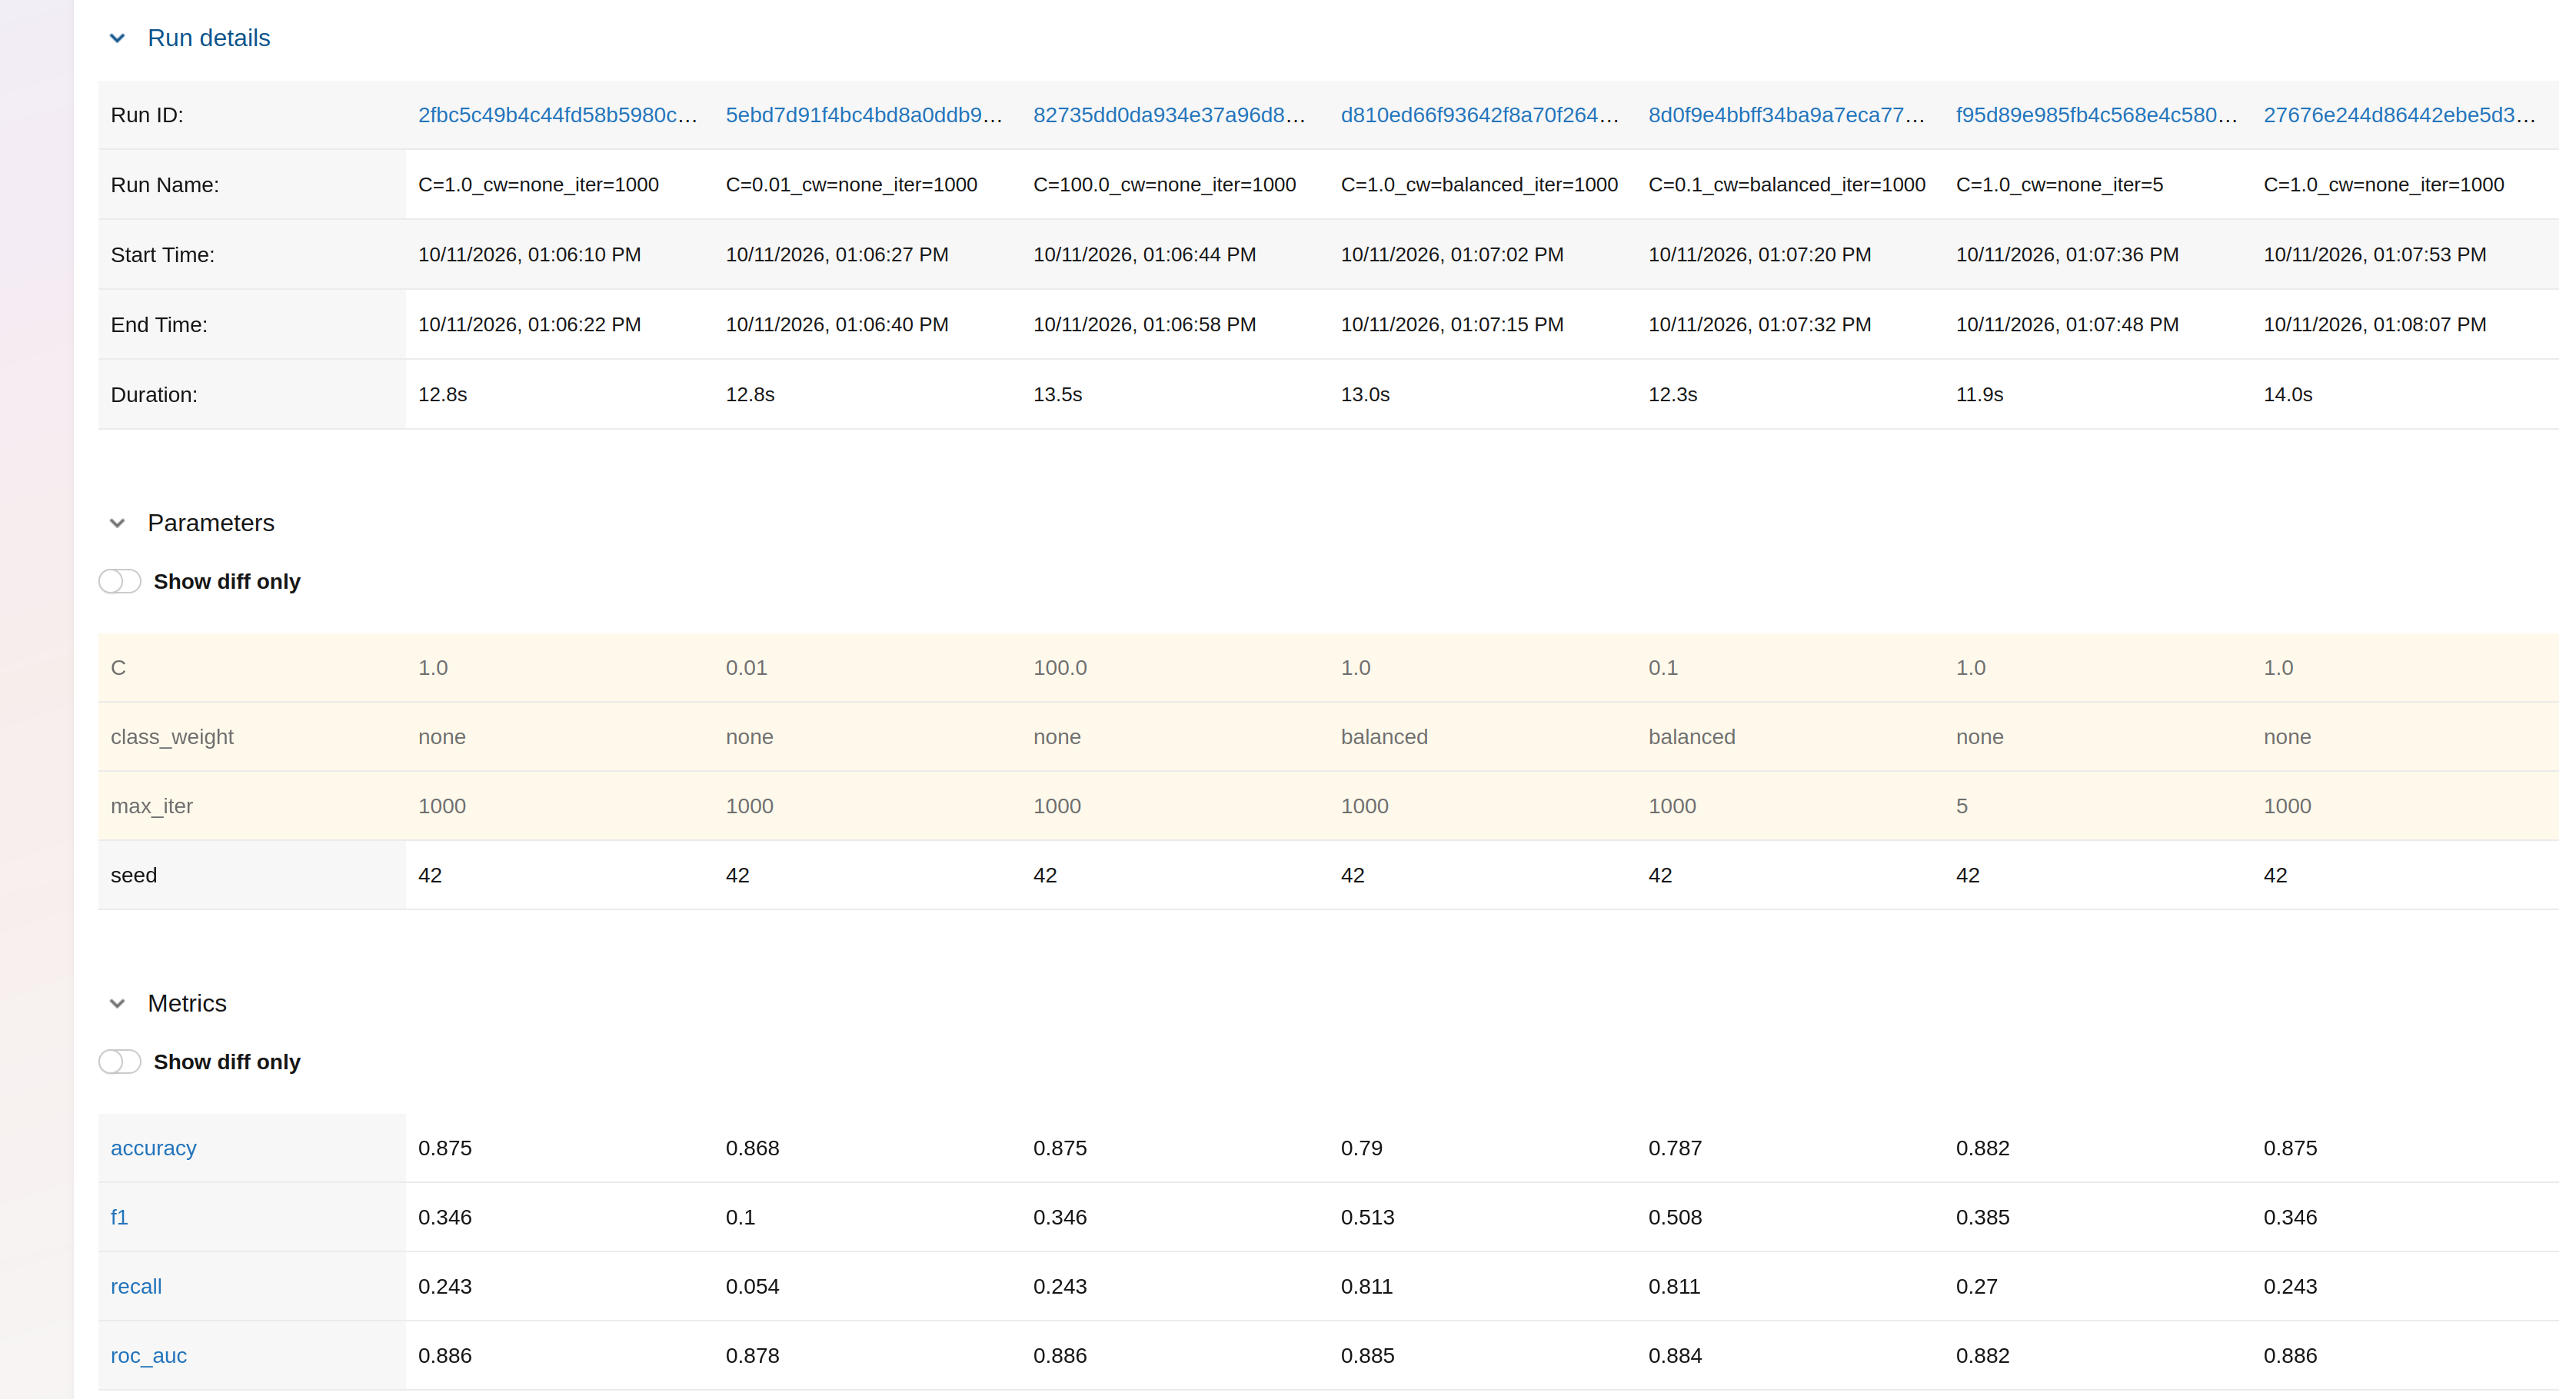
\includegraphics[width=\linewidth]{figures/05_mlflow_tabla_comparativa.png}
\caption{Tabla comparativa de MLflow con los parámetros y las métricas de las
siete corridas.}
\end{figure}

\Needspace{14\baselineskip}
\section*{Declaración de uso de herramientas de inteligencia artificial}

En esta entrega se utilizó Claude Code de Anthropic, con el modelo Claude Opus 5.5, para la
generación parcial de código, orientada a mejorar el código propuesto y a plantear
alternativas basadas en decisiones de optimización.

\referencia{Anthropic. (2026). \textit{Claude Code (Claude Opus 5.5)} [Modelo de lenguaje
grande], utilizado para generación parcial de código, mejora del código propuesto y
alternativas de optimización. \url{https://claude.com/claude-code}}

\Needspace{16\baselineskip}
\section*{Referencias}

\referencia{Cortez, P., Cerdeira, A., Almeida, F., Matos, T. y Reis, J. (2009). Modeling wine
preferences by data mining from physicochemical properties. \textit{Decision Support Systems,
47}(4), 547--553. \url{https://doi.org/10.1016/j.dss.2009.05.016}}

\referencia{DrivenData. (s.\,f.). \textit{Cookiecutter Data Science}. Recuperado el 11 de
octubre de 2026, de \url{https://cookiecutter-data-science.drivendata.org/}}

\referencia{MLflow. (s.\,f.). \textit{MLflow Tracking} [Documentación]. Recuperado el 11 de
octubre de 2026, de \url{https://mlflow.org/docs/latest/ml/tracking/}}

\referencia{Pedregosa, F., Varoquaux, G., Gramfort, A., Michel, V., Thirion, B., Grisel, O.,
Blondel, M., Prettenhofer, P., Weiss, R., Dubourg, V., Vanderplas, J., Passos, A., Cournapeau,
D., Brucher, M., Perrot, M. y Duchesnay, E. (2011). Scikit-learn: Machine learning in Python.
\textit{Journal of Machine Learning Research, 12}, 2825--2830.}

\end{document}
